\documentclass[conference]{IEEEtran}

\usepackage{graphicx}

\begin{document}
\title{Non-Photorealistic rendering using edge aware filters}
\author{Parla Surendra Mani kumar\\Nadiminti Praveen \\ Jagarlamudi Sai Laxman}
\maketitle

\begin{abstract}
	Our project aims to create a cartoon effect to the given input image. This was achieved using edge aware filters.	
\end{abstract}

\begin{IEEEkeywords}
	NPR, Bilater filter, image abstraction,domain transfer
\end{IEEEkeywords}

\section{introduction} \label{s1}
 Non-photorealistic rendering (NPR) is an area of computer graphics that focuses on enabling a wide variety of expressive styles for digital art. The input to a two dimensional NPR system is typically an image or video. The output is a typically an artistic rendering of that input imagery (for example in a watercolor, painterly or sketched style).In our project we wish to accomplish this by using edge aware filters. Edge aware filters blurs the image without effecting the edges. 
  
 \section{General Idea}
 The general idea of how it is implemented is as follows:
 \begin{enumerate}
 \item The given image is converted from rgb to lab colour space
 \item L channel of the image is smothened using an edge aware filter
 \item The smothened L channel is then quantized to different levels and an image I1 is created, as a cartoon has few colours.
 \item The smothened L-channel is passed through an edge detection filter for detecting edges and an image I2 is created, as a cartoon highlights edges.
 \item The images I1 and I2 are combined to form modified L-channel.
 \item The modified L-channel and unmodified a,b channel is used to created our required rgb image.
 \end{enumerate}
  Figure \ref{fig:Idea} represents the basic idea of cartoonization.
  
\begin{figure}
 	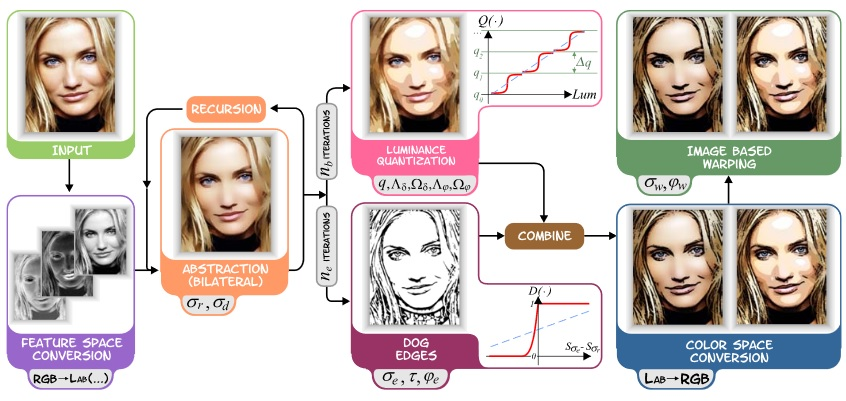
\includegraphics[width = \linewidth]{Idea.jpg}
 	\caption{Idea of Cartoonization}
 	\label{fig:Idea}
 \end{figure}
 
 \section{Edge aware filtering}
 \subsection{Normalized convolution}
Filtering the non-uniformly sampled signal $I_w(ct(x))$ in $\Omega_w$ can be seen as filtering a uniformly sampled signal with missing samples (Figure 8, left). This scenario has been studied by Knutsson and Westin [1993] in the context of data uncertainty, where they showed that optimal filtering results, in the mean square sense, are obtained by normalized convolution (NC). For a uniform discretization $D(\Omega)$ of the original domain $\Omega$, NC describes the filtered value of a sample $p \in D(\Omega)$ as
$$J(p) = \frac{1}{K_p}\sum_{q \in D(\Omega)}I_qH(t(\hat{p}),t(\hat{q}))$$
where $K_p = \sum_{q \in D(\Omega)}H(t(\hat{p}),t(\hat{q}))$  is a normalization factor for p, and $t(\hat{p}) = ct(p)$. For N samples and an arbitrary kernel H, the cost of evaluating is $O(N^2 )$. However, as ct(x) is monotonically increasing, we use an efficient moving-average approach [Dougherty 1994] to perform NC with a box filter in O(N) time. The box kernel is defined as
$$H(t(\hat(p)),t(\hat(q))) = \delta{|t(\hat(p)) - t(\hat(p))| \leq r}$$ 
where $r = \sigma_H \sqrt{ 3}$ is the filter radius, and $\delta$ is a boolean function that returns 1 when its argument is true, and 0 otherwise. This box kernel has a constant radius in $\Omega_w$, but a space-varying and non-symmetric radius in $\Omega$, where its size changes according to the similarity between p and its neighborhood in the image manifold MI.. This can be interpreted as an estimate of which neighbors belong to the same population as p. The box kernel is then a robust estimator of the population mean, with connections to robust anisotropic diffusion and bilateral filtering.
 Figure \ref{fig:NC_sample}Filtering in the transformed domain. (Left) Normalized convolution (NC). (Center) Interpolated convolution (IC). (Right) Their interpretation: NC box kernel in blue, IC box kernel in red.\\
 The cost of evaluating Equation 1 using the box kernel from Equation 2 is linear in the number of samples. 
 
 \begin{figure}
 	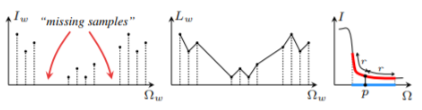
\includegraphics[width = \linewidth]{NC_sample.png}
 	\label{fig:NC_sample}
 \end{figure}
 
 
 
 \subsection{Interpolated convolution}
  Another option when dealing with irregularly sampled data is to use interpolation for approximating the original continuous function
[Piroddi and Petrou 2004]. . Filtering Lw is performed by continuous convolution:
$$J(p) = \int_{\Omega_w}L_w(x)H(t(\hat(p)),x) dx$$
where H is a normalized kernel. Interpolated convolution has an
interesting interpretation: a linear diffusion process working on the
Signal. Implementation For a box filter,the above equation can be evaluated
for all pixels in O(N) time. This is achieved by a weighted moving average
. The normalized box kernel is given by
$$H(t(\hat(p)),x) = \delta{|t(\hat(p))-x| \leq r}/2r$$

where $r = \sigma_H \sqrt{3}$ is the filter radius. Substituting it in above equation.

$$ J(p) = \frac{1}{2r}\int_{t(\hat(p))-r}^{t(\hat(p))+r} L_w(x) dx $$

The linearly-interpolated signal Lw does not need to be uniformly
resampled, since the area under its graph can be explicitly computed
using the trapezoidal rule.


  \subsection{Recursive filtering}
  	Filtering is an important and much used discipline in image processing. The goal is either to remove unwanted components such as noise, or to enhance certain features, or simply as an artistic modification. As we are discussing about fast edge aware filtering approaches, recursive filtering is one of them.Recursive filters are more efficient than straight convolutions even with moderate kernel sizes. A simple blur with a 125x125 pixels kernel, if implemented in a naive way, would be extremely slow even with today's advanced hardware. Recursive filters can handle such a situation dramatically faster.Let us talk about actual implementation of recursive filters.
For a discrete signal I[n] = I(xn),  non edge-preserving filtering can be performed using a 1st-order recursive filter as 

$$J[n] = (1 - a)  I[n] + a J[n - 1] $$

where $a \in [0, 1]$ is a feedback coefficient. Usually IIR filters have recursive feedback system.This filter has an infinite impulse response (IIR) with exponential decay: an impulse of magnitude m at position i generates a response of magnitude $m (1 - a) a^(j - i)$ at $j \geq  i$

Note that j - i can be interpreted as the distance between samples $x_i$ and $x_j$ , 
assuming a unitary sampling interval. Based on this observation, a recursive edge-preserving filter can be defined in the transformed domain as 

$$J[n] = (1 - a^d ) I[n] + (a^d *J[n - 1]) $$

where $d = ct(x_n) - ct(x_{n-1})$ is the distance between neighbor samples $x(n)$ and x(n-1) in the transformed domain . As d increases, a d goes to zero, stopping the propagation chain and, thus,preserving edges.This can be interpreted as a geodesic propagation on the image lattice. The impulse response of equation(2) is not symmetric, since it only depends on previous inputs and outputs (it is a causal filter). A symmetric response is achieved by applying the filter twice: for a 1D signal, equation(2) is performed left-to-right (top-to bottom) and then right-to-left (bottom-to-top). The feedback coefficient of this filter is computed from the desired filter variance as $a = \exp^{(-\frac{ \sqrt{2}}{\sigma_H})}$ can be derived as follows
\\
The continuous equivalent of the recursive kernel is \\
$f(x) = (1-a)a^x$, $x \in [0,\infty)$ , $ a\in (0,1)$;\\
where x represents the distance between samples and a is the feedback coefficient. f(x) is not normalized since\\
$$\int_0^\infty f(x)dx = - \frac{1-a}{\log(a)}$$
Normalizing f we obtain $f(x) = -\log(a)a^x$.The first and second moments of f are, respectively:
$$<f> = -\log(a) \int_0^\infty xa^xdx = -\frac{1}{\log(a)}$$
$$<f^2> = -\log(a) \int_0^\infty x^2a^xdx = -\frac{2}{\log(a)^2}$$
The variance of f is then given by 
$$Var(f) = <f^2>-<f>^2 = \frac{1}{\log(a)^2}$$
Since the signal is filtered twice with f(left-to-right and right-to-left), the total variance of the filter is 2 Var(f). Given the desired variance$\sigma_H^2$:
$$\sigma_H^2 = 2Var(f) = \frac{2}{\log(a)^2}$$
we solve for a and find \\
$a = \exp(-\frac{\sqrt{2}}{\sigma_H})$ and $a = \exp(-\frac{\sqrt{2}}{\sigma_H})$\\
where the former is our solution since $a \in (0,1)$

\begin{figure}
 	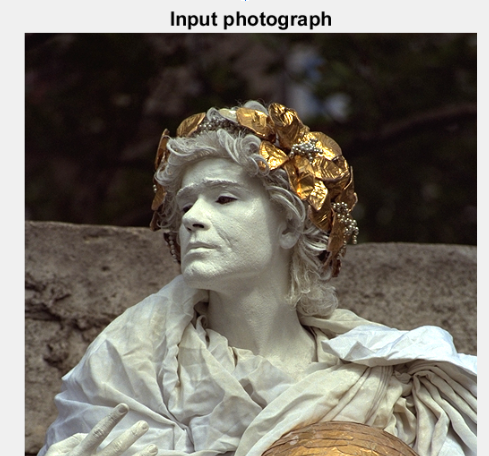
\includegraphics[width = \linewidth]{input_image.png}
 	\caption{Input image}
 \end{figure}
 
 \begin{figure}
 	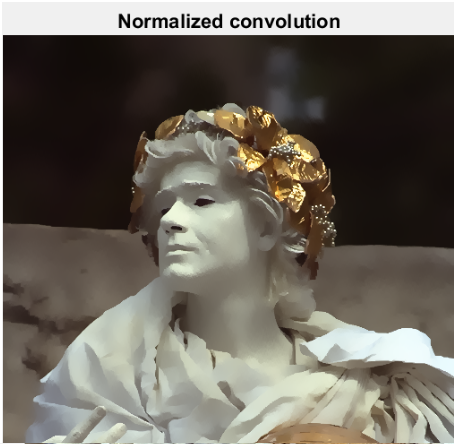
\includegraphics[width = \linewidth]{NC_output.png}
 	\caption{NC output}
 \end{figure}
 
 \begin{figure}
 	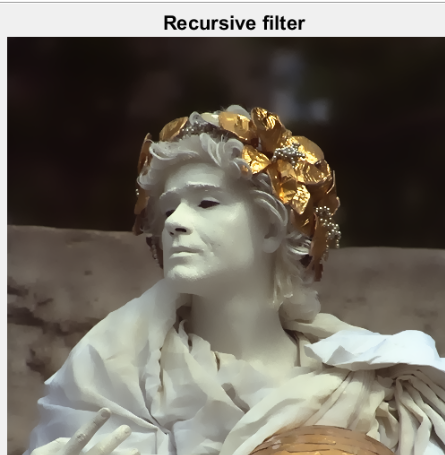
\includegraphics[width = \linewidth]{RF_output.png}
 	\caption{RF output}
 \end{figure}
 
  \begin{figure}
 	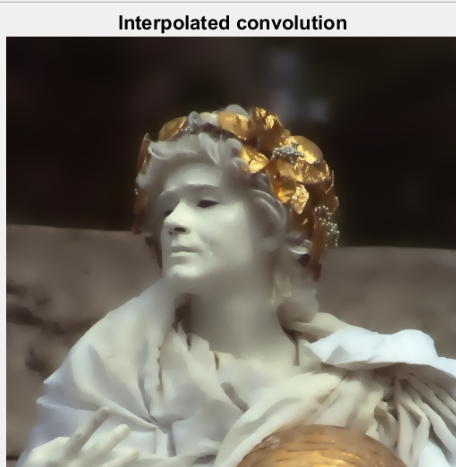
\includegraphics[width = \linewidth]{IC_output.png}
 	\caption{IC output}
 \end{figure}
 
 \section{DoG edges}
 	A computationally simple approximation is the difference-of-Gaussians(DoG) operator.we define our DoG edges using a slightly smoothed step function. The parameter $\tau$ in the equation 4 gives amount of center-surround difference required for cell activation, and $\phi_e$ controls the sharpness of the activation falloff. In the following, we define $S_{\sigma_e} = S(x,\sigma_e)$ and $S_{\sigma_r} = S(x,\sqrt{1.6}\sigma_r)$.
 	$$D(x,\sigma_e,\tau,\phi_e) = 1  if   (S_{\sigma_e}-\tau.S_{\sigma_r}) > 0$$
 	$$D(x,\sigma_e,\tau,\phi_e) = 1+\tanh(\phi_e.(S_{\sigma_e}-\tau.S_{\sigma_r}))  otherwise$$
 	$$S(y,\sigma_e) = \frac{1}{2\pi\sigma_e^2}\int f(x)c(y-x,\sigma_e) dx $$
 	Here,$\sigma_e$ determines the spatial scale for edge detection. The larger the value, the coarser the edges that are detected. The threshold level $\tau$ determines the sensitivity of the edge detector. For small values of $\tau$ , less noise is detected, but real edges become less prominent.As$\tau$ approaches 1, the filter becomes increasingly unstable. We use $\tau=0.98$ throughout.  The falloff parameter,$\phi_e$, determines the sharpness of edge representations, typically $\phi_e \in [0.75,5.0]$. For $n_b$ bilateral iterations, we extract edges after $n_e<n_b$ iterations toreduce noise.Typically, $n_e \in {1,2}$ and $n_b \in {3,4}$.
 
 \section{Results}
 Figure \ref{fig:inputCartoon} represents the input for cartoon.
 Figure \ref{fig:outputCartoon} represents the output for cartoon.
 
 \begin{figure}
 	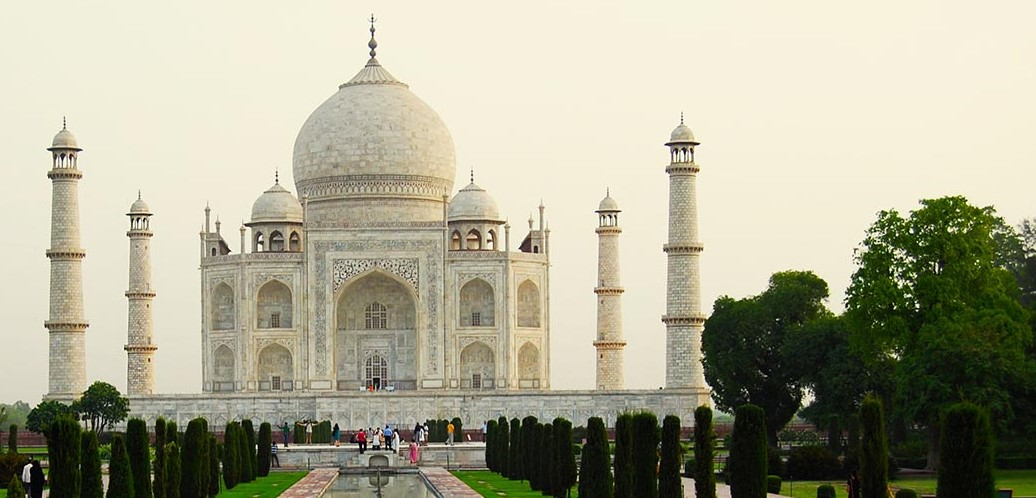
\includegraphics[width = \linewidth]{taj.jpg}
 	\caption{input image for cartoonization}
 	\label{fig:inputCartoon}
 \end{figure}

  \begin{figure}
 	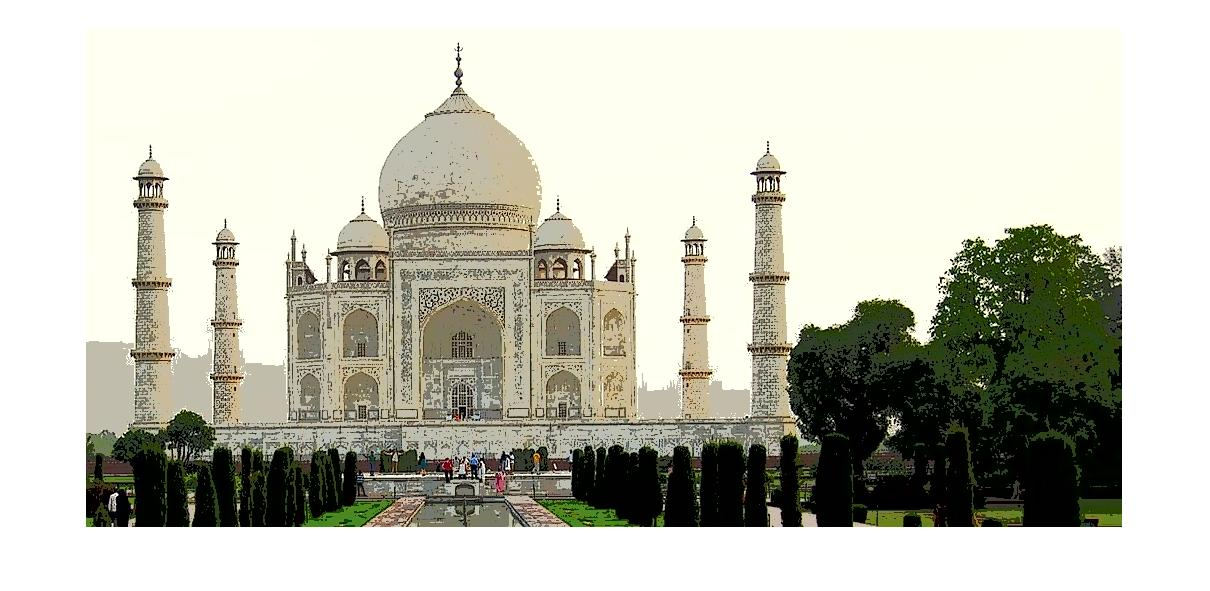
\includegraphics[width = \linewidth]{taj_out.jpg}
 	\caption{output for cartoonization}
 	\label{fig:outputCartoon}
 \end{figure}
 
 \section{Limitations}
 As most other fast edge-preserving filters, our 2D filters are not rotationally invariant (i.e., filtering a rotated image and rotating a filtered image may produce different results). This behaviour may cause problems for applications that rely on content matching
Our 1D edge-preserving filters can be applied to other kinds of signals and to higher-dimensional data. Other possible directions for exploration involve applying our filters on meshes, and their implementation in the frequency domain.

 
 \section{Conclusion and future work}
We have presented a new approach for performing high-quality edge-preserving filtering of images. Our solution is based on a transform that defines an isometry between curves on the 2D image manifold in 5D and the real line. This transform preserves the geodesic distance between points on the curve, adaptively warping the input signal so that 1D edge-preserving filtering can be efficiently performed in linear time. We demonstrated three realizations for our 1D edge-preserving filters, based on normalized convolution, interpolated convolution, and recursion. These filters have very distinct impulse responses, making each one more appropriate for specific application.

\section{Acknowledgement}
We would like to thank Professor Saumik Bhattacharya for their insightful lectures which helped alot for successful completion of the project. 

\end{document}
